\chapter{Usecases}
\label{sec:usecases}
%
\section{Parameter narrowing}
% 
\begin{itemize}
    \item myelin radius
    \item micro oder macro
    \item dn -> trel
    \item voxelsize
    \item n filter rho
    \item intensity
    \item LAP pixel size
\end{itemize}
% 
% \begin{figure}[!tbh]
%     \centering
%     \resizebox{.95\textwidth}{!}{
%     % \inputtikz{gfx/test.tikz}
%     }
% 	\caption{test_plot}
% 	\label{fig:test_plot}
% \end{figure}
% 

\subsection{single fiber f}
\begin{align*}
    f(\alpha, \varphi) &= f(-\alpha, \varphi + \pi)\\
    f(\alpha, \varphi) &= f(\alpha+2\pi, \varphi)  = f(\alpha, \varphi+2\pi)\\
\end{align*}
\begin{align*}
    S:(f(\alpha, \varphi)) \rightarrow (\mathbb{R}, [0, 2 \pi), [0, 1)))\\
    S(f(\alpha, \varphi)) = S(f(\alpha, \varphi - \Delta\varphi)) + \begin{pmatrix}0\\ \Delta \varphi\\ 0\end{pmatrix}\\
    S(T(f(\alpha, \varphi), \theta, \phi) = S(T(f(\alpha+, \varphi+), -\theta, -\phi)
\end{align*}
% 
\subsection{two fiber population}
\begin{align*}
    S(f_0(\alpha, \varphi), f_1(\omega, \psi)) = \\
    T(S(f_0(\alpha, \varphi), f_1(\omega, \psi)), \theta, \phi) = 
\end{align*}
% 
% \begin{figure}[!tb]
%     \resizebox{\textwidth}{!}{
%     \inputtikz{gfx/model/sphere_discretization.tikz}
%     }
% 	\caption{sphere\_discretization}
% 	\label{fig:sphere_discretization}
% \end{figure}
% % 
% \begin{figure}[!tb]
%     \resizebox{\textwidth}{!}{
%     \inputtikz{data/5/voxel_size_vs_diff_dir.tikz}
%     }
% 	\caption{voxel\_size\_vs\_diff\_dir}
% 	\label{fig:voxel_size_vs_diff_dir}
% \end{figure}
% 
%  MACHT PROBLEME FIXME:
% \begin{figure}[!tb]
%     \resizebox{\textwidth}{!}{
%     \inputtikz{data/5/voxel_size_vs_retardation.tikz}
%     }
% 	\caption{voxel\_size\_vs\_retardation}
% 	\label{fig:voxel_size_vs_retardation}
% \end{figure}
% 
\begin{figure}[!tb]
\resizebox{\textwidth}{!}{
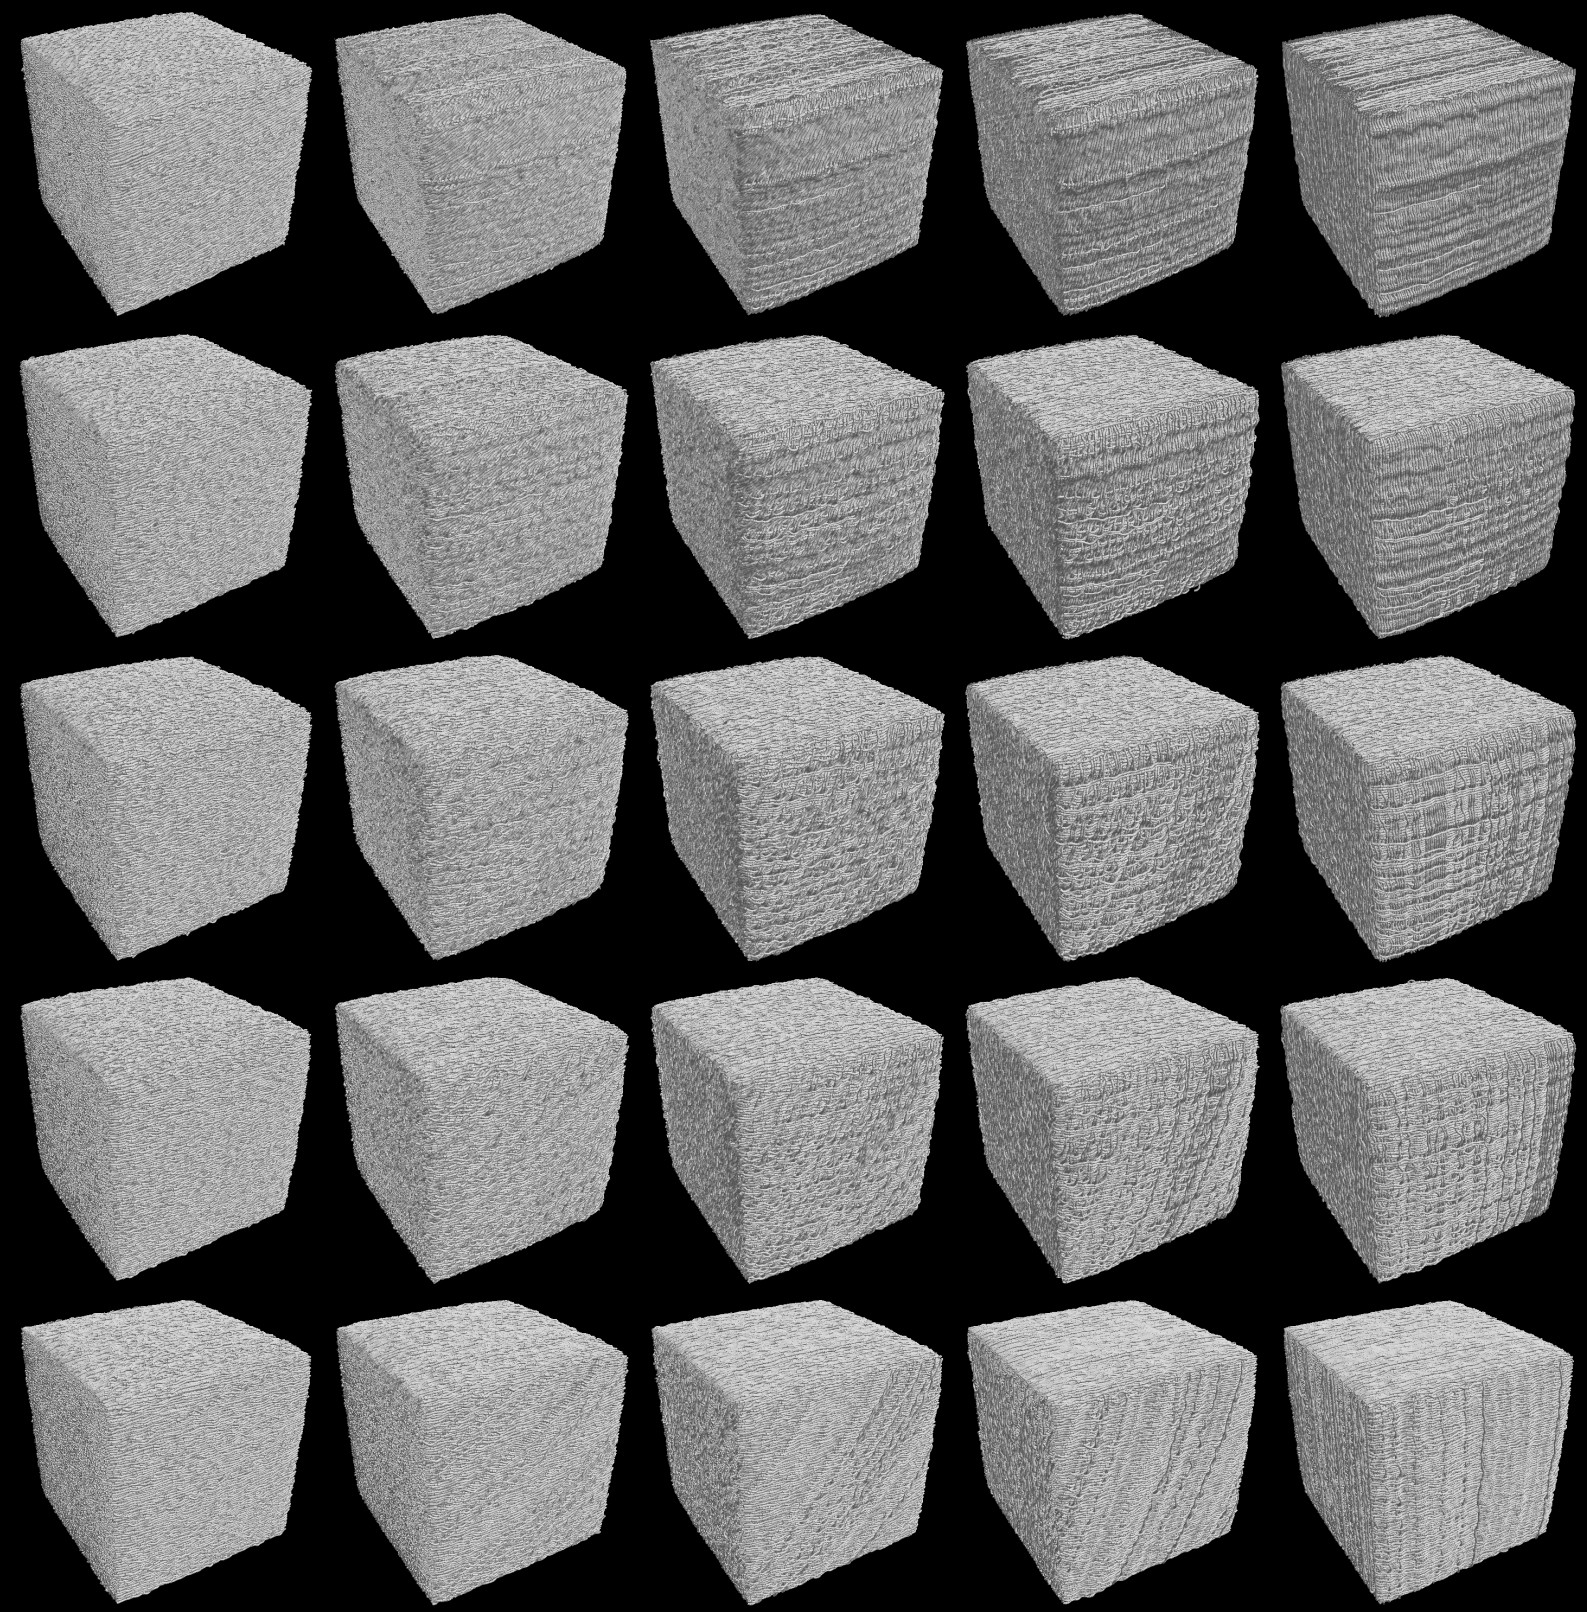
\includegraphics[]{gfx/model/cube_2pop_montage.jpg}
%\begin{minipage}{30cm}
%%\foreach \psi [count=\i] in {0.1, 0.2, 0.3, 0.4, 0.5, 0.6, 0.7, 0.8, 0.9}{
%%	\foreach \omega in {0.0, 10.0, 20.0, 30.0, 40.0, 50.0, 60.0, 70.0, 80.0, 90.0}{	
%\foreach \psi [count=\i] in {0.1, 0.3, 0.5, 0.7, 0.9}{
%    \foreach \omega in {10.0, 30.0, 50.0, 70.0, 90.0}{
%        \includegraphics[trim={110, 70, 90, 130}, clip, width=6cm] %width=2.5cm
%        {dev/data/cube_2pop/cube_2pop_psi_\psi_omega_\omega_.solved.ppm.png}
%        \hspace{-0.5cm}
%    }
%    \vspace{-0.1cm}
%    \ifthenelse{\i<9}{\newline}{}
%}
%\end{minipage}
}
\caption{A test}
\end{figure}
% 
\section{ROFL}
%
\section{Tissue Geometry in Experimental Results}
%
\section{Traktography}
%
\section{ODF}
%
\section{Dispersion}